\section{Introduction}
\label{sec:Introduction}
%wat, waar, waarom
%maatschappelijke bijdrage van het project
The environment is constantly being influenced by humanity and this influence has been debated since the hippie movement in the '60s.
The debate whether humanity puts too much pressure on the environment has only increased in recent years; the full impact of oil-spills and climate change are still being discussed.

This project will focus on an environmental hazards that has recently become apparent: Plastic Soup.
However, the project will not focus on how Plastic Soup affects nature, but how Artificial Intelligence can help to clean up the waste.

%Environment is important, AI can help with the conservation... [oa citeren van \citep{vannature}]


\subsection{Plastic Soup: An environmental problem}
\label{sec:Intro-Plastic Soup}
%Bede context, Maatschappelijke relevantie
%Large amounts of plastic waste ends up in the world's ocean... [oa citeren van \citep{barnes2005drifting}, \citep{moore2011plastic}]
Large amounts of plastic waste end up in the world's oceans and have a significant impact on marine life \citep{barnes2005drifting}.
Plastic Soup or Plastic Ocean are both collective nouns for this environmental problem.
As \citeauthor{barnes2005drifting} indicate, the amount of flotsam in the oceans increases annually as does the increasing proportion of plastic.

When people dispose plastic objects not in trash cans, but near rivers, wind and water flow ensure the objects float through rivers into the ocean.
The currents in the oceans transport the flotsam around the oceans where it settles in patches.
In figure \ref{fig:plastic-where} the estimated location of the Great Pacific Ocean Patch is shown.
Plastic does not decay in nature, therefore a sizeable portion of marine life ingests the plastic after which it ends up in their digestive system. 
Figure \ref{fig:plastic-bird} shows how much plastic can end up in a bird.
In addition to the dangers for marine life, large amounts of plastic end up on beaches, as shown in figure \ref{fig:plastic-beach}.
This has a sizeable impact on local society and economy.

\begin{figure}%[h!bt]
  \centerline{
   \begin{minipage}{\widefigwidth}
 	\begin{center}
     \begin{subfigure}[t]{.65\textwidth}
      \ifx\showfig\undefined
       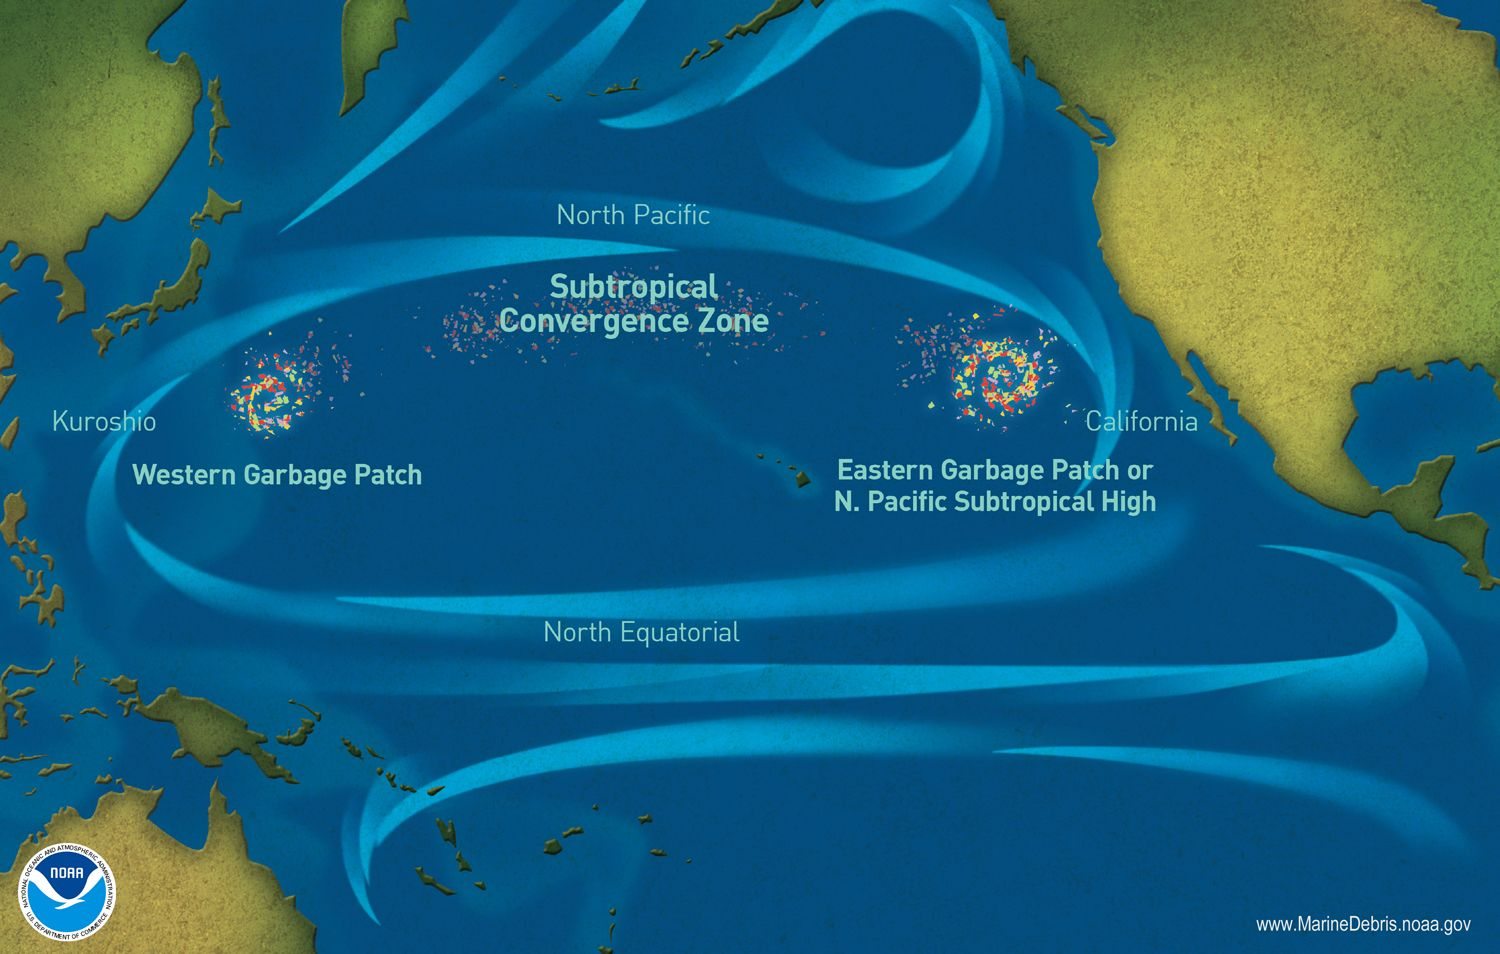
\includegraphics[keepaspectratio=true,width=\textwidth]{images/garbage-patch.jpg} \fi
      \caption{Ocean currents in the Pacific that `collect' the Plastic Soup. Map by NOAA source: \url{http://education.nationalgeographic.com/education/encyclopedia/great-pacific-garbage-patch}}
      \label{fig:plastic-where}
     \end{subfigure}
    \end{center}\\
   \begin{subfigure}[t]{.48\textwidth}
    \ifx\showfig\undefined
	 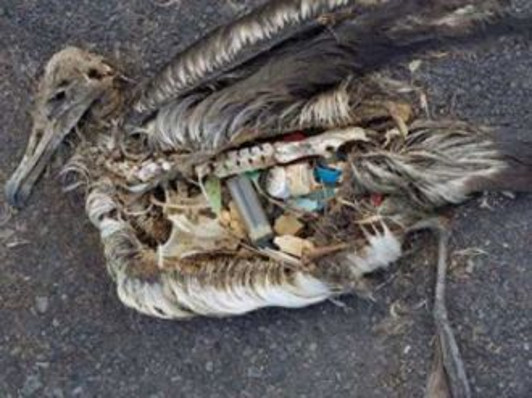
\includegraphics[keepaspectratio=true,width=\textwidth]{images/Bird_with_plastic_stomach.jpg} \fi
	\caption{The stomach contents of a bird that ate plastic. Photograph by Chris Jordan, U.S. Fish and Wildlife Service }
	\label{fig:plastic-bird}
   \end{subfigure}
   \hfill
   \begin{subfigure}[t]{.48\textwidth}
    \ifx\showfig\undefined
	 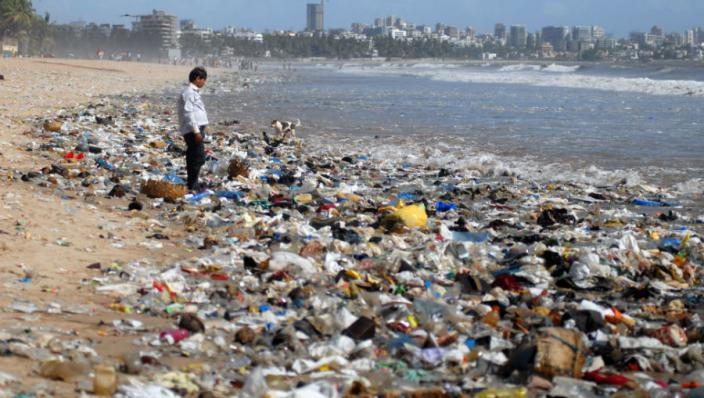
\includegraphics[keepaspectratio=true,width=\textwidth]{images/plastic-beach.jpg} \fi
	\caption{A polluted beach in Mumbai, India. Photograph by EPA }
	\label{fig:plastic-beach}
   \end{subfigure}
   \caption{Three images that show the impact of Plastic Soup on the environment and society.}% (a) shows where the sea-currents deposit the plastic. (b) shows how much plastic can end up in a bird. (c) shows a polluted beach in Mumbai, India.}
   \label{fig:plastic-impact}
   \end{minipage}
  }
\end{figure}

The most significant problem is probably micro-plastic.
When plastic floats in water for some time, sunlight and minerals break the plastic objects down into grains.
These grains of plastic are usually only several micro meters in size and can infect the ecosystem to a large extend \citep{moore2011plastic}.
The full impact of micro-plastic is still unknown, however these plastic grains can end up in bloodstreams of animals and even humans and clog their arteries.

To recapitulate, Plastic Soup can influence the environment to a large extend.
The oceans become polluted with plastic and it kills marine life. Above that society is also influenced and it is even possible that humans die from ingesting micro-plastic.

The pressure of Plastic Soup on the environment has caused several organisations to form in order to address this problem and find solutions for the problem.
The nascency of organisations addressing this problem and searching for solutions have gained media attention and thus cause the growing awareness for the Plastic Soup.
These organisations would benefit of systems that can detect plastic automatically.
Therefore, this project will focus on techniques that are able to distinguish plastic from marine life in ocean water.
The goal of this project is to develop a system based on state-of-the-art techniques that is able to distinguish plastic from animals in images.

\subsection{Project outline}
\label{sec:Intro-Me}
%Onderzoeksvraag, proefopzet, hypothese
To develop a system that can detect plastic, state-of-the-art imaging techniques will be used.
In recent years the accuracy of imaging techniques on object recognition have steadily increased, as section \ref{sec:Theory} describes.
This project will research how these techniques will perform on Plastic Soup detection.

A dataset of annotated images will be constructed to be used in this project.
This dataset can be used to train and test the build system.
To recognise the images containing plastic, a Convolutional Neural Network (CNN) will be used.
The CNN will not be trained on the data itself but a pre-trained network will be used to construct a feature-vector of the image.
These feature-vectors will be used to train a classifier to classify the images in either containing plastic or not containing plastic.
The classifier used in this project is a Support Vector Machine (SVM); to distinguish between plastic and marine-life, two SMVs will be trained.

Both CNNs and SVMs are known to reach high accuracy in Computer Vision, therefore it is hypothesised that this method for plastic recognition should give an appropriate baseline.

Besides the detection of images containing plastic, this project will also research if the location of the plastic within an image can be detected.
As a prove of concept, the pipeline of the plastic recognition will be adapted a small amount to give results for localisation.
%To truly localise the plastic in the image, more research will be necessary.

\subsection{Outline of the thesis chapters}
\label{sec:Intro-Outline}
The performance of the plastic-soup detector created in this project are described in section \ref{sec:Conclusion} with the tables of the results located in section \ref{sec:Results}.
In section \ref{sec:Method} the method of the project is described, section \ref{sec:Data} shows how the data used in this project was acquired, and in section \ref{sec:Discussion} I will go into the parts that can be improved in further research.
But first, in section \ref{sec:Theory} the current state-of-the-art techniques in the field of Computer Vision will be discussed.
%In section \ref{sec:Theory}... \todo{when the thesis is finished, fill this paragraph}















\iffalse
%...dangers of microplastic...

%...big impact on marine life and life in general...

%==Urgentie had groter kunnen worden gemaakt. Hoeveel plastic is er? Wat wordt er al aan gedaan? Hoeveel vogels hebben er last van? Waar komt dat plastic vandaan? Etc.

\subsection{Current solutions}
\label{sec:Intro-Current}


One of the organisations that addresses the problem is Saraswater \citeneed.
This organisation is developing techniques to clean the ocean of this plastic waste.
Saraswater made an apparatus that can be mounted on a ship which shovel the waste from the water.
The small scale experiments that they performed show promising results.

These plastic shovelling ships would benefit from being autonomous.
If no humans are needed, the ships can roam the oceans for many months without the need for visiting harbours.

%One of them is Saraswater. They are developing techniques .. [oa bronnen van de organisaties (niet zozeer artikelen)]
%To help she ships of saraswater, atomise the process with autonomous agents...
%laatse zin: dit is niet genoeg, automatiseering
\subsection{Automation}
\label{sec:Intro-Automate}
When the ships are controlled by an autonomous agent, less human labour is needed for the clean up of the Plastic Ocean.
This project will try to begin with automation of the clean-up.

The automation of the ships is a long term goal.
Before the ships of Saraswater can be autonomous, they first need to `see' to know where the plastic is to clean up.
That is why this project will focus on detecting plastic in ocean water from image data.
Further research expanding this project could develop true autonomous agents controlling the plastic shovelling ships.



%Using state-of-the-art imaging techniques... probably effect... Investigate what will work best by using different algorithms on a dataset of annotated images...


\fi